%%%%%%%%%%%%%%%%%%%%%%%%%%%%%%%%%%%%%%%%%%%%%%%%%%%%%%%%%%%%%%%%%%%%%%
% LaTeX Template: Project Titlepage
%
% Source: http://www.howtotex.com
% Date: April 2011
% 
% This is a title page template which be used for articles & reports.
% 
% Feel free to distribute this example, but please keep the referral
% to howtotex.com
% 
%%%%%%%%%%%%%%%%%%%%%%%%%%%%%%%%%%%%%%%%%%%%%%%%%%%%%%%%%%%%%%%%%%%%%%
% How to use writeLaTeX: 
%s
% You edit the source code here on the left, and the preview on the
% right shows you the result within a few seconds.
%
% Bookmark this page and share the URL with your co-authors. They can
% edit at the same time!
%
% You can upload figures, bibliographies, custom classes and
% styles using the files menu.
%
% If you're new to LaTeX, the wikibook is a great place to start:
% http://en.wikibooks.org/wiki/LaTeX
%
%%%%%%%%%%%%%%%%%%%%%%%%%%%%%%%%%%%%%%%%%%%%%%%%%%%%%%%%%%%%%%%%%%%%%%
%
% --------------------------------------------------------------------
% Preamble
% --------------------------------------------------------------------
\documentclass[paper=a4, fontsize=10pt]{scrartcl}	% KOMA
\usepackage[bottom=1.1in, top=0.9in]{geometry}
\usepackage{lmodern}

\newcommand{\specialcell}[2][c]{%
	\begin{tabular}[#1]{@{}c@{}}#2\end{tabular}}
\usepackage{todonotes}
\usepackage{listings}
\usepackage{graphbox}
\usepackage{hyperref}
\usepackage{twoopt}
\usepackage{adjustbox}
\usepackage[english]{babel}
\usepackage{graphicx}
\usepackage{subcaption}
\usepackage{mwe}
\usepackage{color, colortbl}
\usepackage[protrusion=true,expansion=true]{microtype}	
\usepackage{amsmath,amsfonts,amsthm,amssymb}
\usepackage{tabularx}
\usepackage{float}
\usepackage{tikz} 
\usepackage{xcolor}
\usepackage{listings}
\usepackage{arydshln}
\usepackage{bytefield}


\definecolor{mGreen}{rgb}{0,0.6,0}
\definecolor{mGray}{rgb}{0.5,0.5,0.5}
\definecolor{mPurple}{rgb}{0.58,0,0.82}
\definecolor{backgroundColour}{rgb}{0.95,0.95,0.92}

\newcommand\setrow[1]{\gdef\rowmac{#1}#1\ignorespaces}
\newcommand\clearrow{\global\let\rowmac\relax}
\usepackage{graphicx}
\usepackage[T1]{fontenc}
\definecolor{Red}{rgb}{1,0.7,0.7}
\definecolor{Yellow}{HTML}{FAFAD2}
\definecolor{Green}{HTML}{9ACD32}
\definecolor{Blue}{rgb}{0.5,0.8,1}
\lstset{
	frame=single,
	xleftmargin=15pt,
	xrightmargin=15pt,
	basicstyle=\ttfamily\small
}
\lstdefinestyle{CStyle}{
    backgroundcolor=\color{backgroundColour},   
    commentstyle=\color{mGreen},
    keywordstyle=\color{magenta},
    numberstyle=\tiny\color{mGray},
    stringstyle=\color{mPurple},
    basicstyle=\footnotesize,
    breakatwhitespace=false,         
    breaklines=false,                 
    captionpos=b,                    
    keepspaces=true,                 
    numbers=left,                    
    numbersep=5pt,                  
    showspaces=false,                
    showstringspaces=false,
    showtabs=false,                  
    tabsize=2,
    language=C
}
% --------------------------------------------------------------------
% Definitions (do not change this)
% --------------------------------------------------------------------
\newcommand{\HRule}[1]{\rule{\linewidth}{#1}} 	% Horizontal rule
\newcommandtwoopt*{\myref}[3][][]{%
	\hyperref[{#3}]{%
		\ifx\\#1\\%
		\else
		#1~%
		\fi
		\ref*{#3}%
		\ifx\\#2\\%
		\else
		\,#2%
		\fi
	}%
}

\makeatletter							% Title
\def\printtitle{%						
	{\centering \@title\par}}
\makeatother									

\makeatletter							% Author
\def\printauthor{%					
	{\centering \large \@author}}				
\makeatother							

% --------------------------------------------------------------------
% Metadata (Change this)
% --------------------------------------------------------------------
\title{	\normalsize \textsc{Politecnico di Torino\\GPU Programming} 	% Subtitle
	\\[2.0cm]								% 2cm spacing
	\HRule{0.5pt} \\						% Upper rule
	\LARGE \textbf{\uppercase{Report: PROJECT\\Webcam streaming \& filters}}	% Title
	\HRule{2pt} \\ [0.5cm]		% Lower rule + 0.5cm spacing
	\normalsize 
	\today % Todays date
}

\author{
	Matteo Battilana, Salvatore Gabriele La Greca, Giovanni Pollo
}

\begin{document}
	% ------------------------------------------------------------------------------
	% Maketitle
	% ------------------------------------------------------------------------------
	\thispagestyle{empty}		% Remove page numbering on this page
	
	\printtitle					% Print the title data as defined above
	\vfill
	\printauthor				% Print the author data as defined above
	\newpage


	\thispagestyle{empty}		% Remove page numbering on this page
	\tableofcontents
	\newpage

	% ------------------------------------------------------------------------------
	% Begin document
	% ------------------------------------------------------------------------------
	\setcounter{page}{1}		% Set page numbering to begin on this page
	\section{Introduction}

	A classical video streaming algorithm over internet or over any other communication channel is based on the concept of sending not frame by frame as they are but instead they are based on sending the first frame and then the difference between the new one and the previous, where difference here is to be indended pixel-by-pixel difference.\\
	
	If this can be arguable for video with a lower resolution, the heaviness of sending each frame as it is for high video resolution is notable. Let's take as an example a FULL HD video, means that each frame is composed of 1920x1080 pixels where 1920 is the width of the frame while 1080 is the height. Supposing the frame is in RGB24 format, means that each pixel is rapresented by 3 byte (one for each channel R, G, and B).\\
	
	By doing a rapid computation, each frame measures $3 \cdot 1920 \cdot 1080 B = 6220800 B = 5.93 MB $. Supposing now the video used by example is a 30 fps video, means that each second we have 30 frame, each of one measures 5.93 MB: each second we are sending about 178 MB. To send 178 MB/s we need a transfer link bandwith of 1492 Mbps, that is unfeasible.\\
	
	So the solution is to send the difference, and this means sending only the pixels that change or, better, pixels where their difference is above a certain threshold. \\

	The purpose of the project is to demonstrate the performances that are obtainable by computing the difference on a CPU and to compare them with the ones obtainable by using a General Purpose GPU or \textit{GPGPU}. A Nvidia GPU will be used for the benchmark and therefore the code will be based on CUDA. Among all these considerations, different filters will be added in order to demonstrate the potentiality of GPGPU computations on video elaboration and streaming.

	\section{Video Streaming}
	\label{sec:streaming}

	Before looking at the algorithm that computes the difference between frames, is important to give a look at how frames are captured and the overall architecture of the software. It's a client server architecture where the server transmits the difference to the client via a socket.\\

	All the different variants of implementation that will be analyzed produces three outputs:

	\begin{itemize}
		\itemsep0sp
		\item \texttt{h\_pos}: the number of pixels that are different and greather than a certain threshold.
		\item \texttt{h\_diff}: in code it is actually the array of the current frame that after the application of the algorithm contains the difference of each byte.
		\item \texttt{h\_xs}: it's a mapping vector for the \texttt{h\_diff}. This means that the \texttt{h\_diff[0]} is the difference of byte elemnt at position \texttt{h\_xs[0]}.
	\end{itemize}
	 
	In order to capture frame by frame from the webcam and to visualize them, OpenCV is used. It's not so efficient in terms of performances, especially on the platform used (Nvidia Jetson Nano with 4 ARM cores @ 1.5 GHz) but for the purpose of this project it will be fine. The most important thing to underline is that a frame will be rapresented by the OpenCV's object \texttt{Mat} that contains, among other informations, the dimension of the image (that is fixed to a FULL HD resolution) and an array of \texttt{uint8\_t} items, each representing a channel of a pixel for each pixels of the image. The array can be allocated automatically at the creation of the \texttt{Mat} object or an external array can be used and later on this feature will be exploited.\\

	The aim is to have an efficient software, so a multi thread approach is adopted. There are, in fact, 3 different threads each of them with a different purpose: capture, elaborate and send. They work in a circular way. Means that the capture thread is a producer for the elaborate one, the elaborate one is a producer for the send one and the last one is a producer for the capture one. In this way we have all the threads working at the same time on a different task. The t2 thread is where the magic happens so where the elaboration of the difference is executed.
	
	\begin{center}
		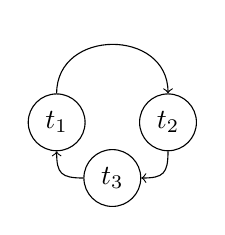
\begin{tikzpicture}[main/.style = {draw, circle}] 
			\node[main] (1) {$t_1$}; 
			\node[main] (3) [below right of=1] {$t_3$}; 
			\node[main] (2) [above right of=3] {$t_2$}; 

			% \draw[->] (1) -- (2);
			\draw[->] (1) to [out=90, in=90, looseness=1.5] (2);
			\draw[->] (2) to [out=270, in=360, looseness=1.5] (3);
			\draw[->] (3) to [out=180, in=270, looseness=1.5] (1);
		\end{tikzpicture} 
	\end{center}

	In the following pages, for metric considerations these terms will be used:

	\begin{itemize}
		\itemsep0sp
		\item \texttt{fps}: number of frames per second.
		\item \texttt{read}: time of execution of the capture thread.
		\item \texttt{for}: time of execution of the elaboration thread. This is what is under discussion in this project.
	\end{itemize}

	\subsection{CPU Implementation}
	The CPU implementation is the easier one and the most basic implementation of the algorithm. It consists on a loop between each byte that compose the two frames (the current one and the previous one) and compute the difference, storing it in a new vector.\\

	The C++ implementation is the following:
	\begin{lstlisting}[style=CStyle]
	int total = 3 * ctx.sampleMat->rows * ctx.sampleMat->cols; // no. bytes
	Mat pvs = pready->pframe->clone();
	pready->h_pos = 0;

	for (int i = 0; i < total; i++) {
		int df = pready->pframe->data[i] - previous.data[i];
		if (df < -LR_THRESHOLDS || df > LR_THRESHOLDS) {
			pready->pframe->data[pready->h_pos] = df;
			pready->h_xs[pready->h_pos] = i;
			pready->h_pos++;
		} else {
			pvs.data[i] -= df;
		}
	}

	previous = pvs;
	\end{lstlisting}

	The code here is pretty simple. For each byte, the difference \texttt{df} is computed. If this difference is greater than a fixed threshold \texttt{LR\_THRESHOLDS} means that it is a valid difference so it can be sent. For all the benchmarks proposed in the following, the value of \texttt{LR\_THRESHOLDS} is fixed to $ 20 $. The result of the reconstructed frame at the client side can be seen at Figure \ref{fig:stream_ok}.\\

	\begin{figure}[H]
		\centering
		\includegraphics[width=0.7\linewidth]{images/streaming_ok2.png}
		\caption{\textit{The result of the reconstructed frame}}
		\label{fig:stream_ok}
	\end{figure}
	
	The important point here is that if the difference is too low, it can't be simply discarded, so a kind of negative feedback is needed. This is the purpose of the line of code at line 7, where the value of the byte of the current frame (that at the end of the loop will be the previous for the next iteration) is itself minus the value of the difference. This means that at the next iteration, if that value changes again and its difference increases it will take under consideration as a big difference. Without this, there will be a sum of errors in the reconstructed image, leading in a wrong visualization. The result if the error is not considered can be seen at Figure \ref{fig:stream_error}.
	
	\begin{figure}[H]
		\centering
		\includegraphics[width=0.7\linewidth]{images/streaming_differror.png}
		\caption{\textit{What happens after a certain time if the error is not take under consideration}}
		\label{fig:stream_error}
	\end{figure}

	The performances here are pretty bad. By means of in-code time measurements, the video streaming is stable at 7 fps with an average \texttt{for} time of 140.0 ms and an average \texttt{read} time of 0.0 ms. This means that here the big bottleneck is due to the elaboration part of the software.

	\begin{figure}[H]
		\centering
		\includegraphics[width=0.8\linewidth]{images/chart1.png}
		\caption{\textit{Pixel Difference Comparison}}
	\end{figure}

	\subsection{GPU Implementation}
	The idea is now to port this in the GPU. The GPU can be seen as an accelerator for the CPU, an accelerator that is capable of a high degree of parallelism by executing a lot of simple threads all in parallel in a SIMD way.\\

	In order to port this in CUDA and execute the computation on the GPU, a series of considerations needs to be done. First of all, it's not said that by executing this in GPU there is a direct improvement in performance. This is due to the fact that there is a big bottleneck between the CPU and the GPU and this is the bus that connects them. A GPU in order to do some work on some data needs to have them in its memory (so the GPU can't access directly the CPU's RAM).\\

	The first thing to do, before defining the kernel (the piece of code that is offloaded to the GPU), is to understand how split the 6220800 bytes among the concurrent threads of the GPU. In the Mat object, the frame is rapresented row-major, means that rows are at consecutive address, as shown in Table \ref{tab:row_major}.

	\begin{table}[H]
		\centering
		\begin{tabular}{ |c:c:c| } 
			\hline
			0 & 1 & 2 \\
			\hdashline
			3 & 4 & 5 \\ 
			\hdashline
			6 & 7 & 8 \\ 
			\hline
		\end{tabular}
		\begin{tabular}{ |c|c|c|c|c|c|c|c|c| } 
			\hline
			0 & 0 & 0 & 0 & 0 & 0 & 0 & 0 & 0 \\
			\hdashline
			0x0 & 0x1 & 0x2 & 0x3 & 0x4 & 0x5 & 0x6 & 0x7 & 0x8 \\
			\hline
		\end{tabular}
	\caption{\textit{Row major rapresentation in memory}}
	\label{tab:row_major}
	\end{table}

	Threads can be organized differently according how they access the memory, and in this case there can be two possible cases of memory access per thread:

	\begin{table}[H]
		\parbox{.45\linewidth}{
			\centering
			\begin{tabular}{l|ccc}
				Thread 0 & 0 & 3 & 6\\
				\hline
				Thread 1 & 1 & 4 & 7\\
				\hline
				Thread 2 & 2 & 5 & 8\\
			\end{tabular}
			\caption{Non consecutive access}
		}
		\hfill
		\parbox{.45\linewidth}{
			\centering
			\begin{tabular}{l|ccc}
				Thread 0 & 0 & 1 & 2\\
				\hline
				Thread 1 & 3 & 4 & 5\\
				\hline
				Thread 2 & 6 & 7 & 8\\
			\end{tabular}
			\caption{Consecutive access}
		}
	\end{table}
	
	So the entire array can be divided into <N> chunks where <N> is the number of threads to launch on the GPU. By organizing the kernels in a way they can access the memory in a consecutive access, the kernel will achieve the so called \textit{memory coalesced access}.\\

	How many threads? For a first implementation, and in order to have a modular implementation of the code (so it can be executed on different GPUs with different capabilities), the following code is adopted:

	\begin{lstlisting}[style=CStyle]
	struct cudaDeviceProp prop;
	cudaGetDeviceProperties(&prop, 0); // retrieves device infos

	int total = 3 * ctx.sampleMat->rows * ctx.sampleMat->cols; // no. bytes
	int nMaxThreads = prop.maxThreadsPerBlock;
	int maxAtTime = total / nMaxThreads;
	\end{lstlisting}

	According to this, each thread will work on $N = \textit{maxAtTime}$ consecutive bytes, dividing the memory into \textit{nMaxThreads} chunks, and overlapping is totally avoided. The GPU used for the experiments allows a maximum of 1024 threads to be executed concurrently.\\

	For what concerns the memory allocation, obviously the CPU address space and the GPU one are two separated things, so a specific allocation on the device side must be done. This can be accomplished thanks to some CUDA's API as follows:

	\begin{lstlisting}[style=CStyle]
	uint8_t *d_current, *d_previous, *d_diff;
	int *d_xs;
	unsigned int *d_pos;

	cudaMalloc((void **)&d_diff, total * sizeof *d_diff);
	cudaMalloc((void **)&d_xs, total * sizeof *d_xs);
	cudaMalloc((void **)&d_current, total * sizeof *d_current);
	cudaMalloc((void **)&d_previous, total * sizeof *d_previous);
	cudaMalloc((void **)&d_pos, sizeof *d_pos);
	\end{lstlisting}


	\subsubsection{Naif version}

	The naif version of the implementation is to port as it is the CPU code into a kernel. From the host side (the CPU) that asks to the device (the GPU) to execute the kernel, there are three kind of operations to be done:

	\begin{enumerate}
		\itemsep0sp
		\item copy the frame into the GPU's memory
		\item launch the kernel
		\item copy back the results from the GPU's memory to the HOST memory
	\end{enumerate}

	In the naif implementation, both the previous and current frames are copied into the GPU's memory. At the end of the execution, the results are copied back. This implies 2 transfers HostToDevice (HtoD) for current and previous and 3 transfers DeviceToHost (DtoH) for h\_xs, h\_diff and h\_pos. A memset on the device side is required too to set the initial value of d\_pos to 0.\\

	The host will therefore execute the following operations:

	\begin{lstlisting}[style=CStyle]
cudaMemset(d_pos, 0, sizeof *d_pos);

// launch
cudaMemcpy(d_previous, previous.data, total, cudaMemcpyHostToDevice);
cudaMemcpy(d_current,pready->pframe->data,total,cudaMemcpyHostToDevice);
kernel<<<1,nMaxThreads>>>(d_current,d_previous,d_diff,maxAtTime,d_pos,d_xs);

// copy back
cudaMemcpy(pready->pframe->data, d_diff, total, cudaMemcpyDeviceToHost);
cudaMemcpy(pready->h_xs, d_xs, total*sizeof *d_xs, cudaMemcpyDeviceToHost);
cudaMemcpy(&pready->h_pos, d_pos, sizeof *d_pos, cudaMemcpyDeviceToHost);

// copy previous
cudaMemcpy(previous.data, d_current, total, cudaMemcpyDeviceToHost);
	\end{lstlisting}

	It's possible to notice a pretty similar structure of the CPU implementation, where the \textit{for loop} is replaced by the kernel. The kernel is launched with a grid dimension of (1, 0, 0) and a block dimension of (\textit{nMaxThreads}, 0, 0), thus only the x dimension is used because the kernel is coded in such a way that the chunk assigned to it is analyzed in a linear way. \\
	
	In order to define the code of the kernel, there are two main problems to be analyzed first:

	\begin{enumerate}
		\itemsep0sp
		\item How does the kernel knows at which address it must work?
		\item How is possible to fill a variable size array in a concurrent environment in CUDA?
	\end{enumerate}

	The first problem is easily solved, it's only a matter of indexes. Each kernel needs to know which chunk of the memory is assigned to it so first of all it computes it's own unique index that will space from 0 to $nMaxThreads - 1$. Once this is defined, the kernel knows that it must work on the i-th chunk but this needs to be translated into the real index to be used to address the memory. Because each size is \textit{maxAtTime} large, means that the the real index that identifies the start of the chunk is $ threadIndex \cdot maxAtTime$.\\

	The second problem is a bit more complicated to solve. In the CPU implementation a variable h\_pos is used in order to indicize the resulting vectors an incremental way and at the end this variable is used to know the length of the result. The problem when this concept is trasposed to the GPU world is that there is a global variable d\_pos that is used by \textit{nMaxThreads} concurrently so there is the need to read and increment this variable in a safe way, so only a kernel at a time can ready and modify it. Luckly, the CUDA framework offers a series of functions that ensures atomic operations between kernels, and in this case the needed one is \texttt{atomicInc(unsigned int *address, unsigned int val)} where \textit{address} is the pointer to the value that needs to be atomic incremented, \textit{val} is the wraparound value, so the max value that the variable can reach before going again to 0, and it returns as result the value atomically incremented.\\

	After solved those problems, a look at the real implementation of the kernel can be given:
	
	\begin{lstlisting}[style=CStyle]
__global__ void kernel(
uint8_t *current, uint8_t *previous, uint8_t *diff, 
int maxSect, unsigned int *pos, int *xs) {
	int x = threadIdx.x + blockDim.x * blockIdx.x;
	unsigned int npos;
	int df;


	int start = x * maxSect;
	int max = start + maxSect;

	#pragma unroll
	for (int i = start; i < max; i++) {

		df = current[i] - previous[i];
		if (df < -LR_THRESHOLDS || df > LR_THRESHOLDS) {
			npos = atomicInc(pos, 6220801);
			diff[npos] = df;
			xs[npos] = i;
		} else {
			current[i] -= df;
		}

	}

}
	\end{lstlisting}

	As can be seen, apart the computation of the start and end index of the computation, the for loop is pretty much the same as the CPU implementation. The only difference is the one concerting the use of the \texttt{atomicInc} function as explained before.\\

	The performances here are slightly better than the CPU implementation. The video streaming is elaborated at around 13 fps with an average \texttt{for} time of 70.0 ms and an average \texttt{read} time of 0.0 ms, and the comparison with the previous case can be seen in Figure \ref{fig:chart2}. 

	\begin{figure}[H]
		\centering
		\includegraphics[width=0.8\linewidth]{images/chart2.png}
		\caption{\textit{Pixel Difference Comparison}}
		\label{fig:chart2}
	\end{figure}

	This means that the big bottleneck is still due to the elaboration part of the software. Using the profiler offered by Nvidia \textit{nvprof} executed for 30 seconds, it's possible to get a lot more details about the time required by each GPU operation, and in particular what concerns this project is the transfer time and the kernel execution time. The results are shows in table \ref{tab:nvprof_naif}.

	\begin{table}[H]
		\centering
		\begin{tabular}{||c | c c c||} 
			\hline
			Operation & Avg (ms) & Min (ms) & Max (ms) \\ [0.5ex] 
			\hline\hline
			Kernel & 40.295 & 35.912 & 47.033 \\ 
			\hdashline
			DtoH & 4.2975 & 1.5100 & 52.878 \\
			\hdashline
			HtoD & 3.3280 & 2.4544 & 25.808 \\
			\hdashline
			Memset & 0.0008 & 0.0007 & 0.0017 \\
			\hline
		\end{tabular}
		\caption{Profiling results}
		\label{tab:nvprof_naif}
	\end{table}

	\subsubsection{Asynchronous APIs and removal of useless operations}

	In the previous implementation, a big portion of the execution time is covered by the kernel execution but the two data transfers are not negligible. The total average time is about 46 ms means that the \textit{for} time is for the 60\% due to the GPU computation and the remaining part is related to host taks.\\

	CUDA offsers a variant of the APIs that are asynchronous with respect to the device execution. This means that when one of these APIs is called, the operation starts on the device side but the control returns immediately to the host despite the end of the operation on the GPU.\\

	This means that is possible to give to the device a series of operations to execute and meanwhile the host can work on its own operations. In this specific case the host doesn't have any task to complete so a function \texttt{cudaDeviceSynchronize()} is used to wait for the device to complete its operations. Howewer this solution is slightly more efficient because is possible to assign to the GPU all the jobs in a consecutive way then waiting instead of assign a job at a time.

	\begin{lstlisting}[style=CStyle]
cudaMemsetAsync(d_pos, 0, sizeof *d_pos);

cudaMemcpyAsync(d_previous, previous.data, total, cudaMemcpyHostToDevice);
cudaMemcpyAsync(d_current,pready->pframe->data,total,cudaMemcpyHostToDev);
kernel<<<1,nMaxThreads>>>(d_current,d_previous,d_diff,maxAtTime,d_pos,d_xs);

cudaMemcpyAsync(pready->pframe->data, d_diff, total,cudaMemcpyDeviceToHost);
cudaMemcpyAsync(pready->h_xs,d_xs,total*sizeof *d_xs,cudaMemcpyDevToHost);
cudaMemcpyAsync(&pready->h_pos,d_pos,sizeof *d_pos, cudaMemcpyDeviceToHost);

cudaMemcpyAsync(previous.data, d_current, total, cudaMemcpyDeviceToHost);
cudaDeviceSynchronize();
	\end{lstlisting}


	Another optimization that can be done is to remove a particular useless copy both HtoD and DtoH, and that is the one regarding the previous frame. In fact, after the first launch of the kernel, the previous frame is already stored in the GPU's memory so it's avoidable the back copy to the host and gain to the device. What can be done is to implement a simple pointer swap, in fact after the first execution the current frame will become the previous frame at the next round. So there is a pool of two pointers that alternatively works one as the current and the other one as the previous.\\

	The host code becomes like this:

	\begin{lstlisting}[style=CStyle]
// current-previous swap
uint8_t *d_prev = d_current;
d_current = d_previous;
d_previous = d_current;

cudaMemsetAsync(d_pos, 0, sizeof *d_pos);

// Copy in the current pointer and run 
cudaMemcpyAsync(d_current,pready->pframe->data,total,cudaMemcpyHostToDeve);
kernel<<<1,nMaxThreads>>>(d_current,d_previous,d_diff,maxAtTime,d_pos,d_xs);

cudaMemcpyAsync(pready->pframe->data,d_diff,total,cudaMemcpyDeviceToHost);
cudaMemcpyAsync(pready->h_xs,d_xs,total*sizeof *d_xs,cudaMemcpyDevToHost);
cudaMemcpyAsync(&pready->h_pos,d_pos,sizeof *d_pos,cudaMemcpyDeviceToHost);

cudaDeviceSynchronize();
	\end{lstlisting}

	Another optimization in terms of copies regards the download of the two arrays forming the result. In fact, instead of copying all the \textit{total} bytes is smarter to cpy only \textit{d\_pos} bytes, the ones that are really useful.\\

	So the first download copy regards \textit{d\_pos}, then a \texttt{cudaDeviceSynchronize()} is executed in order to wait for the complete of all the previous operation and getting a valid \textit{d\_pos}, then the remaining data are copied. \\
	
	The host code becomes:

	\begin{lstlisting}[style=CStyle]
// current-previous swap
uint8_t *d_prev = d_current;
d_current = d_previous;
d_previous = d_current;

cudaMemsetAsync(d_pos, 0, sizeof *d_pos);

// Copy in the current pointer and run 
cudaMemcpyAsync(d_current,pready->pframe->data,total,cudaMemcpyHostToDeve);
kernel<<<1,nMaxThreads>>>(d_current,d_previous,d_diff,maxAtTime,d_pos,d_xs);

cudaMemcpyAsync(&pready->h_pos,d_pos,sizeof *d_pos,cudaMemcpyDeviceToHost);
cudaDeviceSynchronize();

cudaMemcpyAsync(pready->pframe->data,pready->h_pos,total,cudaMemcpyDToHt);
cudaMemcpyAsync(pready->h_xs,d_xs,pready->h_pos*sizeof *d_xs,cdMemcpyDToH);


cudaDeviceSynchronize();
	\end{lstlisting}

	Last but not least, the \textit{cudaMemsetAsync} at line 6 can be removed completely. In fact, it's possible to move the initial reset of the \textit{d\_pos} counter by doing it at the beginning of the kernel and it's easily done even in a concurrent environment by letting only one kernel to perform the reset. This can be achieved by putting a condition on the kernel index. In this case it will be done by the first kernel. In order to have all the kernel executing more or less in parallel the same instructions, after the reset of the counter, a \texttt{\_\_syncthreads()} is executed that assures that all threads are synchred untill that point. \\

	Thus, the kernel code becomes:

	\begin{lstlisting}[style=CStyle]
__global__ void kernel(
uint8_t *current, uint8_t *previous, uint8_t *diff, 
int maxSect, unsigned int *pos, int *xs) {
	int x = threadIdx.x + blockDim.x * blockIdx.x;
	unsigned int npos;
	int df;

	// counter reset done by thread with index = 0
	if (!x) *pos = 0;
	__syncthreads();


	int start = x * maxSect;
	int max = start + maxSect;

	#pragma unroll
	for (int i = start; i < max; i++) {

		df = current[i] - previous[i];
		if (df < -LR_THRESHOLDS || df > LR_THRESHOLDS) {
			npos = atomicInc(pos, 6220801);
			diff[npos] = df;
			xs[npos] = i;
		} else {
			current[i] -= df;
		}

	}

}
	\end{lstlisting}

	All these optimizations let achieve a big result in performance terms. The video streaming is elaborated at around 20 fps with an average \texttt{for} time of 55.0 ms and an average \texttt{read} time of 0.0 ms, and the comparison with the previous case can be seen in Figure \ref{fig:chart3}. 

	\begin{figure}[H]
		\centering
		\includegraphics[width=0.8\linewidth]{images/chart3.png}
		\caption{\textit{Pixel Difference Comparison}}
		\label{fig:chart3}
	\end{figure}

	The results of the \textit{nvprof} profiler are shown in Table \ref{tab:nvprof_naif2} and is noticeable the big improvement in terms of performances for what concerns the DtoH transfer. The HtoD transfer remains more or less the same but it's executed only one time instead of two as the naif implementation.

	\begin{table}[H]
		\centering
		\begin{tabular}{||c | c c c||} 
			\hline
			Operation & Avg (ms) & Min (ms) & Max (ms) \\ [0.5ex] 
			\hline\hline
			Kernel & 41.426 & 37.278 & 46.423 \\ 
			\hdashline
			DtoH & 0.0227 & 0.0009 & 9.2925 \\
			\hdashline
			HtoD & 3.7813 & 2.1733 & 14.188 \\
			\hline
		\end{tabular}
		\caption{Profiling results}
		\label{tab:nvprof_naif2}
	\end{table}

	\subsubsection{Pinned or page-locked memory}

	Untill now a good bottleneck has been removed and it is the transfer from the Device to the Host. What about the Host to Device transfer? In order to solve this issue an understanding on how memory is managed by the CPU and how the GPU transfers data from the CPU's managed memory and the GPU.\\

	What a modern operating system does is to manage the physical memory through the concept of pages and thus the virtual memory. The address space of the virtual memory is different from the physical one, thus a translation is needed. In order to let the hardware translate from a space to another, a special hardware called translation lookaside buffer (TLB) is used. It's a memory cache that is used to reduce the time taken to access a user memory location and it's part of the chip's memory-management unit (MMU) needed in fact by all the modern operating systems. The TLB stores the recent translations of virtual memory to physical memory and can be called an address-translation cache.\\

	When a CUDA's memcpy is invoked, the DMA starts transfering data but as soon as the translation is not anymore stored in the cache, the operating system has to solve this situation by loading a new page. Thus this is not really a asynchronous operation and it's highly cpu-dependent. Thus the velocity of the copy is based on the speed of the CPU and in edge devices where the CPU is not so performant as a desktop CPU the overhead of this mechanism can't be neglected.\\
	
	The solution is to allocate a piece of memory that is pinned or \textit{page locked}. Executing an allocation like this is like telling the operating system virtual memory manager that the memory pages must stay in physical ram so that they can be directly accessed by the GPU across the PCI-express bus. And it's a lot faster thanks to the DMA: when the memory is page locked, the GPU DMA engine can directly run the transfer without requiring the host CPU, which reduces overall latency and decreases transfer times.\\

	CUDA offers an API to do this, called \texttt{cudaMallocHost()} that works similar to \texttt{cudaMalloc()} but allocates a page-locked memory on the host side. It's required for arrays like \texttt{h\_xs} and \texttt{pready->pframe->data}. If it's pretty easy to be done for \texttt{h\_xs} that is an array directly managed by the code, how is possible to do that for the pframe's data that is something managed by OpenCV? As said at the beginning, the \textit{Mat} object offers a good option, the one to select an external pointer as data array.\\

	\begin{lstlisting}[style=CStyle]
uint8_t *h_frame;
cudaMallocHost((void **)&h_frame, total * sizeof *h_frame);
cudaMallocHost((void **)&pready->h_xs, total * sizeof *pready->h_xs);

// init of Mat object with page-locked h_frame ptr
pready->pframe = new Mat(ctx.sampleMat->rows,ctx.sampleMat->cols,
		ctx.sampleMat->type(), h_frame); 
	\end{lstlisting}

	Without touching anything else, this optimization is able to achieve a good result. The video streaming is elaborated at around 22 fps with an average \texttt{for} time of 43.0 ms and an average \texttt{read} time of 0.0 ms, and the comparison with the previous case can be seen in Figure \ref{fig:chart4}. 

	\begin{figure}[H]
		\centering
		\includegraphics[width=0.8\linewidth]{images/chart4.png}
		\caption{\textit{Pixel Difference Comparison}}
		\label{fig:chart4}
	\end{figure}

	The results of the \textit{nvprof} profiler are shown in Table \ref{tab:nvprof_naif3} and is noticeable the big improvement in terms of performances for what concerns the HtoD transfer. In fact, it's about 1/4 the original one.

	\begin{table}[H]
		\centering
		\begin{tabular}{||c | c c c||} 
			\hline
			Operation & Avg (ms) & Min (ms) & Max (ms) \\ [0.5ex] 
			\hline\hline
			Kernel & 43.386 & 38.093 & 49.607 \\ 
			\hdashline
			DtoH & 0.0102 & 0.0008 & 1.0466 \\
			\hdashline
			HtoD & 0.6740 & 0.6096 & 2.2818 \\
			\hline
		\end{tabular}
		\caption{Profiling results}
		\label{tab:nvprof_naif3}
	\end{table}

	\subsubsection{Kernel global memory access: the cherry on the cake}
	\label{sec:cherry}

	What remains now to further optimize is the kernel execution time. Doing a bunch of analysis, with a maximum number of threads of 1024 each kernel execute a \textit{for loop} that lasts 6075 iterations. Each iteration access in memory three times in the most of the cases (supposing $ N_{pixelChanged} \ll N_{pixelNotChanged} $) and accesses in global memory are a real bit bottleneck for CUDA's kernel because usually the Global memory access time is $400 \sim 600$ cycles. Obviously, each byte needs to be esaminated so it's not possible to randomly cut accesses in memory. How this can be optimized?\\

	The answer to this question is very simple but at the same time it's brilliant: by increase the size of each read or write in memory. By applying this concept, both the memory accesses and the loop iterations are reduced, so it's an optimization in both ways.\\

	The first think to do is to rewrite the kernel in order to support this. The idea is to load into some GPU's registers some bytes regarding a portion of the current and previous frame under consideration by the for loop of a kernel. Then there is always need of a byte-wise substraction and comparison so a inner for loop will access byte-wise the word loaded into the register(s) and will do its computations.\\

	The multi-byte memory access is done using the dynamic pointer cast feature, casting the vector pointers to the data type aimed, Therefore the new kernel implementation, using the most common data type that is the \texttt{int} one, is:

	\begin{lstlisting}[style=CStyle]
typedef int chunk_t;

__global__ void kernel2(
uint8_t *current, uint8_t *previous, uint8_t *diff, 
int maxSect, unsigned int *pos, int *xs) {
    int x = threadIdx.x + blockDim.x * blockIdx.x;
    unsigned int npos;
    int df;
    chunk_t cc, pc; // registers storing current copy, previous copy

    if (!x) *pos = 0;
    __syncthreads();

    int start = x * maxSect;
    int max = start + maxSect;

    #pragma unroll
    for (int i = start; i < max; i++) {

        cc = ((chunk_t *)current)[i];
        pc = ((chunk_t *)previous)[i];

        #pragma unroll
        for (int j = 0; j < sizeof cc; j++) {
            df = ((uint8_t *)&cc)[j] - ((uint8_t *)&pc)[j];

            if (df < -LR_THRESHOLDS || df > LR_THRESHOLDS) {
                npos = atomicInc(pos, 6220801);
                diff[npos] = df;
                xs[npos] = (i*sizeof cc) + j;
            } else {
                current[(i*sizeof cc) + j] -= df;
            }

        }

    }

}
	\end{lstlisting}

	The host code changes a little bit because maxAtTime now needs to be divided by the size of the \texttt{chunk\_t} type. Because it's highly probable that the division results in a non integer value, it must be rounded to the nearest greater integer. \\
	
	This means that by rounding up, each thread will overlap with the next thread of a few bytes. Actually it's not a problem because the probability that while the thread \textit{i} writes at the very last bytes of its chunk the thread \textit{i+1} writes at the very beginning of its chunk is very low because each thread is executed in parallel. The only thing that happens is that the computations on a certain amount of bytes is done two times but each time it's done on the same inputs and the result is always the same. In the case of a low probability of two writes at the same time, as discussed, the overhead in managing the concurrent write is lower than the one of adding instructions to check if the thread is writing outside its chunk (about 1 ms of difference in execution time).\\

	\begin{lstlisting}[style=CStyle]
int max4 = ceil(1.0 * maxAtTime / sizeof(chunk_t));

// CUDA APIs call
// ...
kernel2<<<1,nMaxThreads>>>(d_current,d_previous, d_diff, max4, d_pos, d_xs);
// ...
\end{lstlisting}

	The only problem to manage by choosing the path of not adding any check inside the kernel is that the last kernel can write outside the memory. In order to avoid wrong memory accesses, the allocaiton of the memory on the GPU is done by considering this margin. In fact, a thread will write at most \texttt{sizeof(chunk\_t)} bytes outside the memory, so each memory allocation is done by allocating an additional amount of bytes equal to \texttt{sizeof(chunk\_t)} bytes:

	\begin{lstlisting}[style=CStyle]
uint8_t *h_frame;
cudaMallocHost((void **)&h_frame, total * sizeof*h_frame + sizeof(chunk_t));
cudaMallocHost((void **)&pready->h_xs,tot*sizeof*prdy->hxs+sizeof(chunk_t));

// init of Mat object with page-locked h_frame ptr
pready->pframe = new Mat(ctx.sampleMat->rows,ctx.sampleMat->cols,
		ctx.sampleMat->type(), h_frame); 
	\end{lstlisting}

	The results of the \textit{nvprof} profiler are shown in Table \ref{tab:nvprof_naif4} and is noticeable the big improvement in terms of performances for what concerns the Kernel execution time. In fact, it's almost the 50\% of the previous implementation. The average fps are 21, with a \textit{for} time of 26.0 ms and a \textit{read} time of 30 ms.

	\begin{table}[H]
		\centering
		\begin{tabular}{||c | c c c||} 
			\hline
			Operation & Avg (ms) & Min (ms) & Max (ms) \\ [0.5ex] 
			\hline\hline
			Kernel & 23.700 & 21.590 & 24.671 \\ 
			\hdashline
			DtoH & 0.0079 & 0.0008 & 1.0009 \\
			\hdashline
			HtoD & 0.6483 & 0.6074 & 2.5641 \\
			\hline
		\end{tabular}
		\caption{Profiling results}
		\label{tab:nvprof_naif4}
	\end{table}

	A further optimization can be done by looking at the new kernel implementation and noticing that only 2/3 of the memory accesses are optimized. The feedback write in fact is still done at each byte, and it can be easily optimized by modifying the \texttt{cc} register variable in the inner loop (byte wise) and save back the result in the global memory at the end of the inner loop only if needed (so if the \texttt{cc} variable has been modified).\\
	
	The implementation is the following:

	\begin{lstlisting}[style=CStyle]
typedef int chunk_t;

__global__ void kernel2(
uint8_t *current, uint8_t *previous, uint8_t *diff, 
int maxSect, unsigned int *pos, int *xs) {
    int x = threadIdx.x + blockDim.x * blockIdx.x;
    unsigned int npos;
    int df;
    chunk_t cc, pc; // registers storing current copy, previous copy
    bool currUpdateRequired = false;

    if (!x) *pos = 0;
    __syncthreads();

    int start = x * maxSect;
    int max = start + maxSect;

    #pragma unroll
    for (int i = start; i < max; i++) {

        cc = ((chunk_t *)current)[i];
        pc = ((chunk_t *)previous)[i];

        #pragma unroll
        for (int j = 0; j < sizeof cc; j++) {
            df = ((uint8_t *)&cc)[j] - ((uint8_t *)&pc)[j];

            if (df < -LR_THRESHOLDS || df > LR_THRESHOLDS) {
                npos = atomicInc(pos, 6220801);
                diff[npos] = df;
                xs[npos] = (i*sizeof cc) + j;
            } else {
                ((uint8_t *)&cc)[j] -= df;
                currUpdateRequired = true;
            }

        }

        // storing in global memory only if needed
        if (currUpdateRequired) {
        	((chunk_t *)current)[i] = cc;
        	currUpdateRequired = false;
        }
    }

}
	\end{lstlisting}

	The results of the \textit{nvprof} profiler are shown in Table \ref{tab:nvprof_naif5} and is noticeable another big improvement, reducing the kernel time by another 50\%. The average fps are 24, with a \textit{for} time of 11.5 ms and a \textit{read} time of 40 ms. The overall comparison is shown in Figure \ref{fig:chart5}.

	\begin{table}[H]
		\centering
		\begin{tabular}{||c | c c c||} 
			\hline
			Operation & Avg (ms) & Min (ms) & Max (ms) \\ [0.5ex] 
			\hline\hline
			Kernel & 9.7944 & 8.7887 & 17.906 \\ 
			\hdashline
			DtoH & 0.0080 & 0.0008 & 1.2807 \\
			\hdashline
			HtoD & 0.6443 & 0.5969 & 2.9633 \\
			\hline
		\end{tabular}
		\caption{Profiling results}
		\label{tab:nvprof_naif5}
	\end{table}

	\begin{figure}[H]
		\centering
		\includegraphics[width=0.8\linewidth]{images/chart5.png}
		\caption{\textit{Pixel Difference Comparison}}
		\label{fig:chart5}
	\end{figure}

	The overall situation can be optimized even more. CUDA offers the possibility to perform vectorized memory accesses by using \textit{vectorized data types}. What are them and why they are so important?\\

	First of all, these special data types are of different types depending on their reference type. For example there is \texttt{int2}, \texttt{float3}, \texttt{ulong2} and so on. Looking at the public header files they are defined as follow (taking \texttt{int4} as an example):

	\begin{lstlisting}[style=CStyle]
struct __device_builtin__ __builtin_align__(16) int4 {
    int x, y, z, w;
};

typedef __device_builtin__ struct int4 int4;\end{lstlisting}

	Thanks to the fact they they are \texttt{\_\_device\_builtin\_\_}, they are identified by the CUDA compiler that will optimize the generated instructions by reducing them and using special \textit{vectorized instructions} capable of a larger transaction in the memory. So thanks to these instructions is possible to load big chunks of data at a time with less instructions. Please note that a common struct with 16 int variables as members will not perform well as expected because int4 is a builtin type so recognized by the compiler and vectorized instructions will be used by activating some internal magic in the compiler itself.\\

	The usage of these vectorized instructions is easily seen at the assembly level. The kernel seen before with a classical \texttt{int} data type is translated into these instructions:

	\begin{lstlisting}[style=CStyle]
/*00c8*/ MOV R3, R5;
/*00d0*/ LD.E R18, [R10];
/*00d8*/ LD.E R14, [R2]; 
/*00e0*/ SSY 0x240;      \end{lstlisting}

	The two LD.E instructions are the one corresponding to the two reads from the global memory into the \texttt{cc} and \texttt{pc}. The LD.E is a scalar instruction that will load a word from memory. Using instead \texttt{int4} builtin type, the disassembly code will be:

	\begin{lstlisting}[style=CStyle]
/*00c8*/ MOV R3, R17;        
/*00d0*/ MOV R12, R0;        
/*00d8*/ LD.E.128 R4, [R2];  
/*00e0*/ SSY 0x360;          
/*00e8*/ LD.E.128 R8, [R12]; \end{lstlisting}

	Here, the two LD.E.128 are vectorized instructions. By using the vectorized load and store instructions LD.E.\{64,128\} (and the counter part ST.E.\{64,128\}) operations like load and store data can be done in 64- or 128-bit widths. Using vectorized loads reduces the total number of instructions, reduces latency, and improves bandwidth utilization.\\

	% A small tip. As said these kind of instructions are \textit{vectorized}. They are called in this way because works on a kind of vector and this can be seen in two ways. The first one is looking at the definition of the vectorized type: the \texttt{int4} for example is a struct made of four \texttt{int} so it's a vector of in this sense. Looking at the assembly code instead is possible to see how the two 

	At this point, the \textit{nvprof} profiler is run and the results are shown in Table \ref{tab:nvprof_naif6} and is noticeable a really big improvement in the computation, reducing the kernel time by another 60\%. The average fps are 26, with a \textit{for} time of 4.7 ms and a \textit{read} time of 37 ms. 

	\begin{table}[H]
		\centering
		\begin{tabular}{||c | c c c||} 
			\hline
			Operation & Avg (ms) & Min (ms) & Max (ms) \\ [0.5ex] 
			\hline\hline
			Kernel & 3.4197 & 2.9266 & 9.0223 \\ 
			\hdashline
			DtoH & 0.0061 & 0.0008 & 1.1601 \\
			\hdashline
			HtoD & 0.6387 & 0.5957 & 2.5595 \\
			\hline
		\end{tabular}
		\caption{Profiling results}
		\label{tab:nvprof_naif6}
	\end{table}

	Even if the 128 bit width is the maximum width support, it's possible to optimize the resulting code even more at the instruction level by using a larger builtin types like \texttt{long4}. As can be intuitable, it will be translated into 2 instructions. This helps introducing a slightly optimization by reducing the memory access frequency, achieving an average reduction of 0.4 ms in the kernel execution time.\\

	The resulting assembly code is the following one, where is possible to notice two loads at a time with the first one loading at offset \texttt{0x0} as the normal one and the second one loads at offset \texttt{0x10} that is 128 bit far from the first load, thus with two instructions a total of 256 bit or 32 byte are loaded, that is the size of a \texttt{long4} data type.
	
	\begin{lstlisting}[style=CStyle]
/*00c8*/ MOV R3, R13;
/*00d0*/ LD.E.128 R8, [R20];
/*00d8*/ LD.E.128 R4, [R20+0x10];
/*00e0*/ SSY 0x1e0;
/*00e8*/ LD.E.128 R12, [R2];
/*00f0*/ LD.E.128 R16, [R2+0x10]; \end{lstlisting}
	
	The overall comparison is shown in Figure \ref{fig:chart6}.

	\begin{figure}[H]
		\centering
		\includegraphics[width=0.9\linewidth]{images/chart6.png}
		\caption{\textit{Pixel Difference Comparison}}
		\label{fig:chart6}
	\end{figure}

	In other words, by using \textit{vectorized instructions} the performance improvement comes from efficiency gains, in two ways:

	\begin{enumerate}
		\item At the instruction level, a multi-word vector load or store only requires a single instruction to be issued, so the bytes per instruction ratio is higher and total instruction latency for a particular memory transaction is lower.
		\item At the memory controller level, a vector sized transaction request from a warp results in a larger net memory throughput per transaction, so the bytes per transaction ratio is higher. Fewer transaction requests reduces memory controller contention and can produce higher overall memory bandwidth utilization.
	\end{enumerate}

	% At this point a question could rise: if \texttt{sizeof(int) = 4}, how the correctness of the algorithm is assured even if $ 6075 / 4 $ is not an integer number? 
	
	% TODO: 6075 / 4 is not an int value, what happens?




	% TODO:
	% \begin{itemize}
	% 	\item Copying both previous and current everytime and no fixed page host allocation
	% 	\item Copying only the current and the previous is a swap pointer, still no fixed page host allocation
	% 	\item Page host allocation
	% 	\item Copy of all d\_diff and d\_xs
	% 	\item Copy first d\_pos then a portion of d\_diff and d\_xs according to d\_pos
	% 	\item Access int-by-int
	% 	\item AtomicInc in global memory and in shared memory, there are differences?
	% 	\item Why 512 kernels is best instead of 1024?
	% \end{itemize}

\newpage
\section{Image Text Overlay}

	Another part of the project under discussion is the ability to add a text overlay over an image. In this particular implementation, it supports ASCII characters over a single line of the image. In order to be send over internet, it's executed before applying the algorithm for sent the frame over a socket, according to Chapter \ref{sec:streaming}.\\

	The final result can be seen in Figure \ref{fig:demo_chars}:

	\begin{figure}[H]
		\centering
		\includegraphics[width=0.9\linewidth]{images/chars_ok.png}
		\caption{\textit{Text Overlay}}
		\label{fig:demo_chars}
	\end{figure}

	The basic idea behind the implementation is the ability to generate a frame (made of RGB pixels) of an ASCII character, dynamically and based on an available font. Everything starts from the specification of the supported alphabet. In fact, not all ASCII characters are supported but only a limited set, specified during the compilation time, in order to have an efficient code in terms of memory occupied and execution time without wasting useful resources (both on the host side and on the device side) for characters that are never used.\\

	After defining the alphabet, at the beginning of the program, it's possible to translate each character into a set of pixels composing it. This is done thanks to a series of OpenCV's function like \texttt{cv::getTextSize} that is able to rietrieve the frame dimensions (width and height) of a character and \texttt{cv::putText} that is able to put a text (or a character in this case) over a frame.\\

	First thing that is done is to retrieve the dimension of a character. This is done only for a single character and it is supposed that all the other characters in the alphabet have the same size.\\

	Than, an array storing all the frames one after another is created with a size that is equal to $ n_{chars} \cdot Area_{char} $. A loop on the alphabet will fill this array with all the character' frames. The code to implement this is the following:

	\begin{lstlisting}[style=CStyle]
#define CHARS_STR "0123456789BFPSWbkps :"

auto txtsz = cv::getTextSize("A", cv::FONT_HERSHEY_PLAIN, 3, 2, 0);
int fullArea = 3 * txtsz.area();
	
uint8_t *charsPx = new uint8_t[(sizeof(CHARS_STR) - 1) * fullArea];
memset(charsPx, 0x0, (sizeof(CHARS_STR) - 1) * fullArea);
for (int i = 0; i < (sizeof(CHARS_STR) - 1); i++) {
	Mat pxBaseMat(txtsz.height, txtsz.width, base.type(), charsPx+i*fullArea);
	cv::putText(pxBaseMat, std::string(CHARS_STR).substr(i, 1),
			cv::Point(0, txtsz.height+1), cv::FONT_HERSHEY_PLAIN, 3,
			cv::Scalar(0, 255, 0), 2, cv::LINE_AA);
}\end{lstlisting}

When the array is finally full filled, it's ready to be copied onto the GPU memory. This operation is done only at the beginning, so it's ininfluent from the point of view of the performances:

	\begin{lstlisting}[style=CStyle]
uint8_t *d_charsPx;
int totcpy = fullArea * sizeof *d_charsPx * (sizeof(CHARS_STR) - 1);
cudaMalloc((void **)&d_charsPx, totcpy * sizeof *d_charsPx);
cudaMemcpy(d_charsPx,charsPx,totcpy*sizeof*d_charsPx,cudaMemcpyHostToDev);
\end{lstlisting}

\subsection{GPU Implementation}
After the initialization phase, is now time to give a look at how each character frame is placed onto the image. It's a replacement of the pixels of the frame under analysis with the one of the corresponding character.\\

The first thing to do is to decide how many kernel to launch and how many pixel each kernel needs to manage. By deciding to assign to each kernel a certain number of pixel in a row-major fashion, and by considering the fact that the frame size of each character is fixed but can change if the font is changed, a portion of the code is used to decide in a dynamic way the two values: number of kernels and pixels for each kernel. It's decided by dividing the total number of bytes of a character frame by the number of frame and if it's a multiple of the size of \texttt{chunk\_t} type that for a first analysis will be a \texttt{uint8\_t}, then the number of threads found is the right one. The code is the following:

	\begin{lstlisting}[style=CStyle]
typedef uint8_t chunk_t;

int nThreadsToUse = nMaxThreads;
int eachThreadDoes = 1;
for (int i = nMaxThreads; i > 0; i--) {
	float frac = fullArea / (i * 1.0);
	int frac_int = fullArea / i;
	if ((int)ceil(frac) == frac_int && frac_int % sizeof(chunk_t) == 0) {
		nThreadsToUse = i;
		eachThreadDoes = frac_int / sizeof(chunk_t);
		break;
	}
}
\end{lstlisting}

\subsubsection{Naif version}

After the setup time, its the turn of the computation step. This is the core, where each character of the string to print is analyzed before applying the streaming algorithm. This is done on the host side and not on the device side in order to avoid the copy HtoD of the string.\\

The advantage is given by the usage of async operations, so while the frame is copied on the GPU, the host scans each character and a new kernel is fired in an async way in order to print each character one after the another.

	\begin{lstlisting}[style=CStyle]
// Copy in the current pointer and run 
cudaMemcpyAsync(d_current,pready->pframe->data,total,cudaMemcpyHostToDev);

for (int offset = 0, j = 0; j < text.length(); j++, offset+=txtsz.width*3) {
	int idx;
	for (int i = 0; i < (sizeof(CHARS_STR) - 1); i++) {
		if (CHARS_STR[i] == text.at(j)) {
			idx = i;
			break;
		}
	}

	kernel_char<<<1, nThreadsToUse>>>(d_current, d_charsPx + idx * fullArea,
			eachThreadDoes, offset, 3 * txtsz.width, 3 * pready->pframe->cols);
}
\end{lstlisting}

The basic implementation of the kernel is the following:

	\begin{lstlisting}[style=CStyle]
__global__ void kernel_char(
uint8_t *current, uint8_t *matrix, int N, int offset, 
int matrixWidth, int currWidth) {
    int thid = threadIdx.x + blockIdx.x * blockDim.x;

    int start = thid * N;
    int max = start + N;

    for (int i = start; i < max; i++) {
        int x = offset + i % matrixWidth;
        int y = i / matrixWidth;
        current[y * currWidth + x] = matrix[i];
    } 
	\end{lstlisting}

	By running the profiler for a fixed time of 30 seconds, the kernel takes an average time of 2.981 us so it occupies the 1.53\% of the total time.\\

	A comparison chart is show in Figure \ref{fig:chart7}:

	\begin{figure}[H]
		\centering
		\includegraphics[width=0.9\linewidth]{images/chart7.png}
		\caption{\textit{Text Overlay Comparison}}
		\label{fig:chart7}
	\end{figure}

	\subsubsection{Exploiting the global memory access optimization}

	It's possible then to optimize the kernel from the point of view of the global memory access parallelism as explained in Section \ref{sec:cherry}. By copying and modifing the same kernel structure, the resulting kernel is:

	\begin{lstlisting}[style=CStyle]
typedef long4 chunk_t;

__global__ void kernel2_char(
uint8_t *current, uint8_t *matrix, int N, int offset, 
int matrixWidth, int currWidth) {
    int thid = threadIdx.x + blockIdx.x * blockDim.x;
    chunk_t cc;

    int start = thid * N;
    int max = start + N;

    for (int i = start; i < max; i++) {
        int reali = i * sizeof(chunk_t);
        int x = offset + reali % matrixWidth;
        int y = reali / matrixWidth;

        int idx = (y * currWidth + x) / sizeof(chunk_t);
        cc = ((chunk_t *)current)[idx];

        #pragma unroll
        for (int j = 0; j < sizeof cc; j++) {
            ((uint8_t *)&cc)[j] = matrix[reali + j];
        }

        ((chunk_t *)current)[idx] = cc;
    } 
	\end{lstlisting}

	
	By running the profiler for a fixed time of 30 seconds, the kernel takes an average time of 3.778 us so it occupies the 1.91\% of the total time.\\

	A comparison chart is show in Figure \ref{fig:chart8}:

	\begin{figure}[H]
		\centering
		\includegraphics[width=0.9\linewidth]{images/chart8.png}
		\caption{\textit{Text Overlay Comparison}}
		\label{fig:chart8}
	\end{figure}

	As noticeable, the performance are worse. This is because the intermediate \textit{for loop} can be compacted in a single instruction because it's only an assignment without other operations in the middle. The new kernel is then shorter and faster, as follow:

	\begin{lstlisting}[style=CStyle]
typedef long4 chunk_t;

__global__ void kernel2_char(
uint8_t *current, uint8_t *matrix, int N, int offset, 
int matrixWidth, int currWidth) {
    int thid = threadIdx.x + blockIdx.x * blockDim.x;
    chunk_t cc;

    int start = thid * N;
    int max = start + N;

    for (int i = start; i < max; i++) {
        int reali = i * sizeof(chunk_t);
        int x = offset + reali % matrixWidth;
        int y = reali / matrixWidth;

        int idx = (y * currWidth + x) / sizeof(chunk_t);
        ((chunk_t *)current)[idx] = ((chunk_t *)matrix)[i];
    } 
	\end{lstlisting}

	By running the profiler for a fixed time of 30 seconds, the kernel takes an average time of 1.868 us so it occupies the 1.01\% of the total time. This means that the last version of the kernel is faster than the first one.\\

	A comparison chart is show in Figure \ref{fig:chart9}:

	\begin{figure}[H]
		\centering
		\includegraphics[width=0.9\linewidth]{images/chart9.png}
		\caption{\textit{Text Overlay Comparison}}
		\label{fig:chart9}
	\end{figure}

	\subsubsection{Constant Memory instead of Global Memory: is it worth?}

	Because character frames are basically constant during the execution of the program, is it really necessary to use the global memory or another kind of memory can be exploited? If yes, is it really worth? \\

	For this kind of purposes, CUDA devices offer the so called Constant Memory, that is a piece of memory on the GPU side that is constant. Because it's \textit{constant} from the GPU point of view but it can modified by the Host, it seems to be perfect for this part of the project.\\

	Usually it's large \textit{64 KB} so supposing to have an alphabet whose frames doesn't exceed this memory limit, a constant variable (array) can be declared and initialized as follows:

	\begin{lstlisting}[style=CStyle]
__constant__ uint8_t c_matrix[(sizeof(CHARS_STR) - 1) * 3 * 32 * 28];

uint8_t *c_matrixPtr;
cudaMemcpyToSymbol(c_matrix, charsPx, totcpy);
cudaGetSymbolAddress((void **)&c_matrixPtr, c_matrix);
\end{lstlisting}

Leaving \texttt{kernel2\_chars} as it is and using \texttt{c\_matrixPtr} instead of \text{d\_charsPx} in the kernel call and running the profiler, an unexpected value is returned by the profiler. The exeuction time is almost the same (faster only for a few nanoseconds) than the previous implementation and this is due to two reasons mainly:

\begin{enumerate}
	\item the kernel is instruction-bound and not memory-bound
	\item according to CUDA's programming guide: "\textit{For all threads of a half-warp, reading from the constant cache is as fast as reading from a register as long as all threads read the same address. The cost scales linearly with the number of different addresses read by all threads.}". This means that the shared memory is really faster than the global memory but becuase the kernel is accessing every time a different address, the cost of access increases by reaching the cost of the global memory.
\end{enumerate}

A comparison chart is show in Figure \ref{fig:chart10}:

	\begin{figure}[H]
		\centering
		\includegraphics[width=0.9\linewidth]{images/chart10.png}
		\caption{\textit{Text Overlay Comparison}}
		\label{fig:chart10}
	\end{figure}


\end{document}